\chapter{Экспериментальное исследование оптических частотных гребенок в кристаллических микрорезонаторах} \label{chapt4}

\section{Экспериментальное наблюдение двойных оптических частотных гребенок в резонаторах из $MgF_2$}

\subsection{Генерация двух солитонных оптических гребенок в двух резонаторах на одном цилиндре}

Для одновременное генерации нескольких солитонных оптических гребенок \cite{Pavlov2017} с практически идентичными частотами повторения были разработаны структуры с несколькими резонаторами одинаковой формы, вырезанными на одном кристаллическом цилиндре из $MgF_2$ (рис. \ref{ris:image1}). Структура имеет 5 одинаковых выступов с радиусом кривизны 35 мкм и диаметром 5.68 мм, соответствующему ОСД 12.1 ГГц. Расстояние между соседними выступами 140 мкм. Такой стэк микрорезонаторов был изготовлен острым резцом с радиусом кривизны 4 мкм на станке алмазного точения.

\begin{figure}[ht]
\begin{minipage}[ht]{1\linewidth}
\center{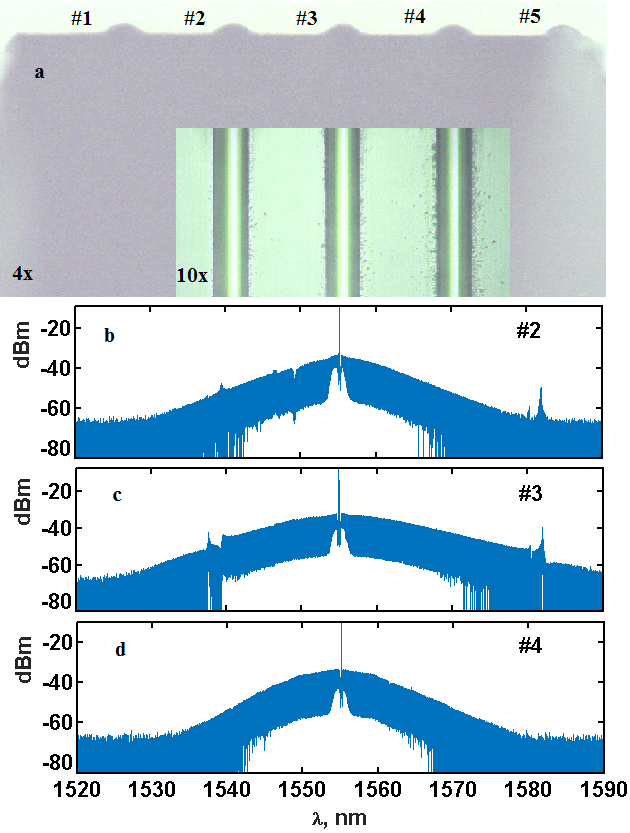
\includegraphics[width=0.75\linewidth]{dual_cavity}}
\end{minipage}
\caption{ (a): Вид резонаторов МШГ на одном кристаллическом цилиндре с диаметром 5.68 мм, радиусом кривизны 35 мкм и расстоянием между соседними выступами 140 мкм. Вставка показывает 3 неотполированные выступа (\#2 -- \#4) сразу после точения, в которых наблюдались солитоны; (b-d): оптический спектр солитонов, генерируемых в 3 различных резонаторах (\#2 -- \#4). Солитонные керровские частотные гребенки имеют ширину $30 - 65$ нм с расстоянием 12.1 ГГц.}
\label{ris:image1}
\end{figure}

Добротность после алмазного точения составила порядка 10$^6$. Сверхвысокая добротность больше $10^9$ была достигнута асимптотическим полированием алмазными суспензиями. В результате финальной полировки разница в ОСД между несколькими выступами была не более 10 МГц, что соответствует разнице в радиусе $0.5 - 1$ мкм в предположении о возбуждении одного семейства мод в обоих резонаторах.

\begin{figure}[ht]
\begin{minipage}[ht]{1\linewidth}
\center{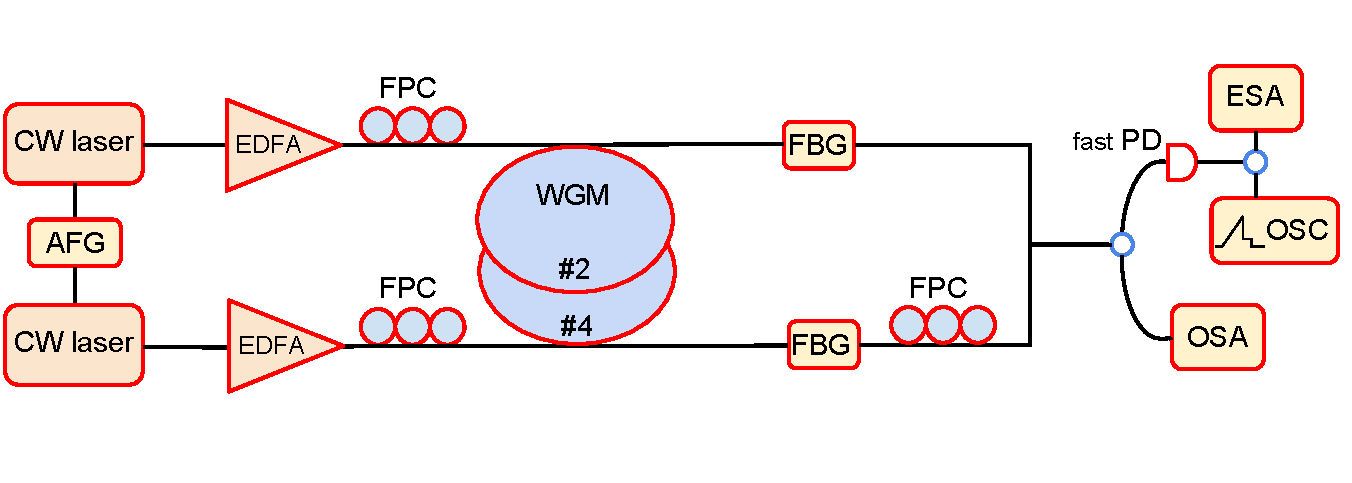
\includegraphics[width=0.75\linewidth]{dual_setup}}
\end{minipage}
\caption{Экспериментальная установка по генерации солитонных двойных гренок из выступов \#2 и \#4. CW: узкополосный перестраиваемый волоконный лазер непрерывной мощности; EDFA: эрбиевый волоконный усилитель; AFG: генератор сигналов произвольной формы; FPC:  волоконный контроллер поляризации; FBG: волоконная Брэгговская решетка; PD: фотодетектор; ESA: анализатор спектра электрических сигналов; OSA: оптический анализатор спектра; OSC: осциллограф.}
\label{ris:image2}
\end{figure}

Схема экспериментальной установке дала на Рис. \ref{ris:image2}.  Два независимых узкополосных волоконных лазера непрерывной мощности Koheras Adjustik ($\lambda \sim 1554$~нм) были усилены в эрбиевом волоконным усилителе связаны с резонаторами через 2 растянутых волокон. Каждое волокно подносится к отдельному выступу микрорезонатора (\#2 и \#4) с противоположных сторон, в которых возбуждаются солитоны с различными ОСД. Генератор сигналов произвольной формы использовался для контроля процесса возбуждения солитонов, подавая одиночный пилообразный импульс. Контроллеры поляризации использовались для оптимизации связи. Волоконная Брэгговская решетка использовались для подавления мощной накачки на выходе после микрорезонатора.

Частоты повторения солитонов наблюдались на быстром фотодетекторе (NewFocus 1014, ширина полосы 25 ГГц) и анализаторе спектра электрических сигналов (Keysight N9030). Для записи оптического спектра использовался оптический спектроанализатор (Yokogawa). На осциллографе наблюдались характерные для солитонов ступеньки в генерируемом свете.

\begin{figure}[ht]
\begin{minipage}[ht]{1\linewidth}
	\center{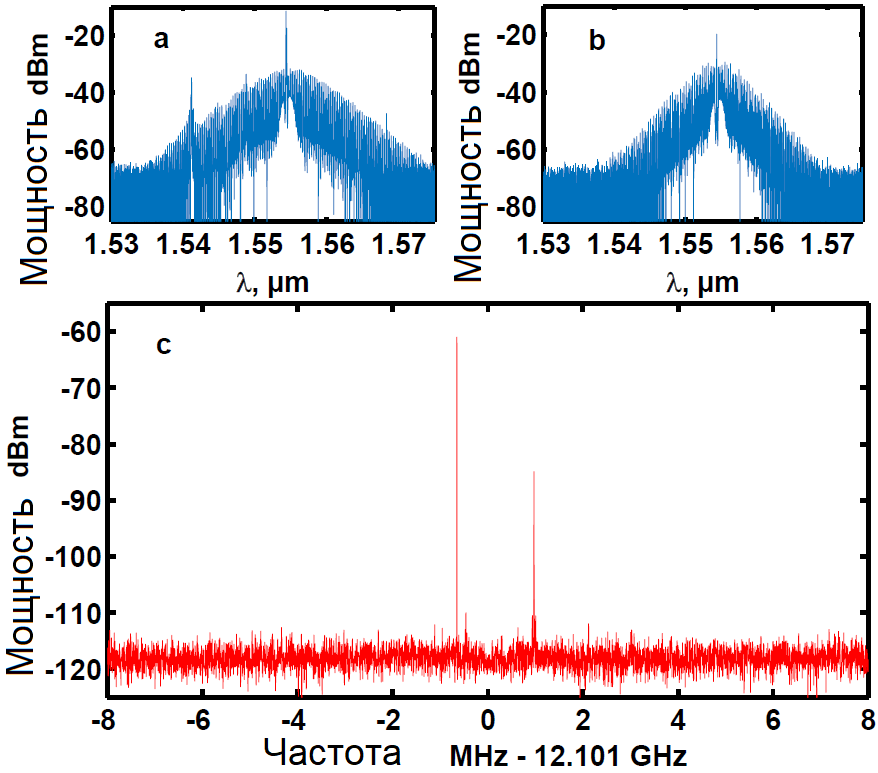
\includegraphics[width=0.5\linewidth]{dual_comb_osa}}
\end{minipage}
\caption{(a-b): Оптические мультисолитонные спектры возбужденные в двух различных резонаторах $\#2$ и $\#4$; (c): сигнал на частоте повторения от двух мультисолитоных состояний, разница в чатотах $1.62$ МГц.}
\label{ris:image3}
\end{figure}

Керровские солитонные гребенки были получены в 3 из 5 резонаторах на 1 цилиндре (Рис. \ref{ris:image1}). Ширина спектра оптических солитонов (Рис.\ref{ris:image1}(b) -- рис.\ref{ris:image1}(d)) составила 30-65 нм около 1554 нм. Разница между частотами лазеров накачки была $8.9-30$ пм. Два потока солитонов с разными частотами повторения $\Delta\mbox{FSR} = \mbox{FSR}_1 - \mbox{FSR}_2 = 1.62$~МГц были одновременно возбуждены в двух выступах на 1 кристаллическом цилиндре и далее сбиты на волоконном делителе. Для настройки на солитоны использовался метод, предложенный в \cite{Herr2014}. Пилообразный однократный сигнал подавался одновременно на оба лазера, начальная точка перестройки выбиралась путем совмещения солитонных ступенек, т.ч. финальная отстройка лазеров попадала в область существования солитонов в обоих резонаторов.

Оптические спектры мультисолитонных гребенок в обоих резонаторах даны на рис.~\ref{ris:image3}(a) -- ~\ref{ris:image3}(b), самая узкая гребенка на рис.~\ref{ris:image3}(b) содержит 350 линий, разделенных на $12.1$ ГГц и покрывает 35 нм около центральной частоты $\lambda = 1554$~нм. Разница в частотах лазеров составила $1.07$~ГГц. Результирующий сигнал биений от двух оптических гребенок переносит двойную гребенку в радиодиапазон (Рис. \ref{ris:image4}), имеет ширину 300 МГц с центром на 1.07 ГГц, содержит 160 линий, разделенных на $1.62$ МГц и имеет огибающую, совпадающую с оптическими профилями двух солитонов. Время жизни двойной гребенки была не более 30 секунд, т.к. не было стабилизации частоты лазера накачки и температуры резонатора.

\begin{figure}[ht]
\begin{minipage}[ht]{1\linewidth}
\center{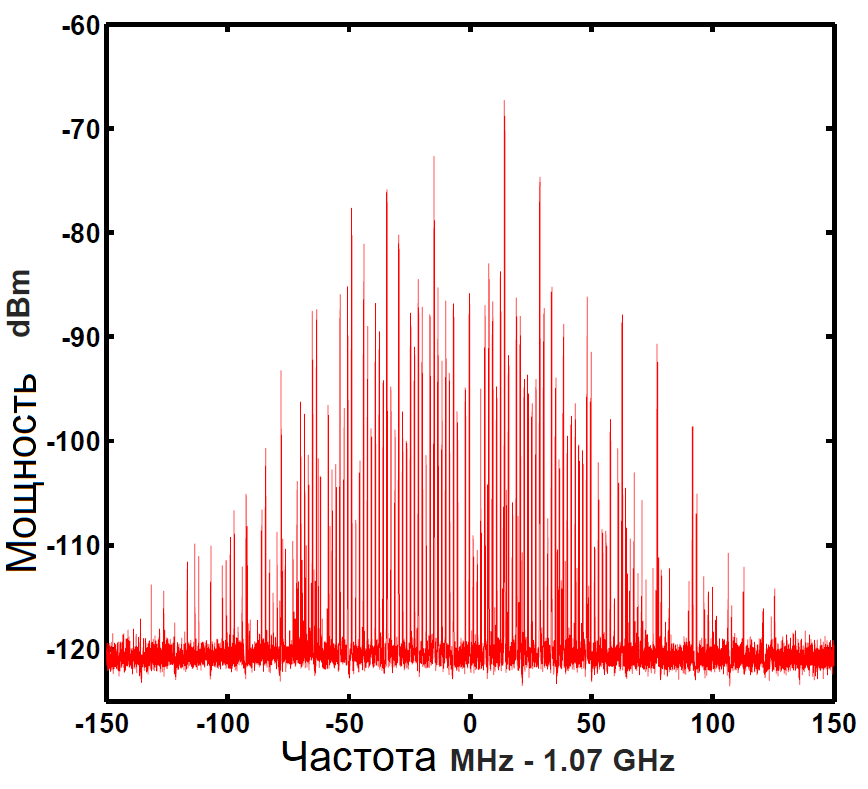
\includegraphics[width=0.5\linewidth]{dual_comb_esa}}
\end{minipage}
\caption{Радиочастотный спектр результата биений двух мультисолитонных керровских оптических гребенок. Радиочастотная двойная гребенка покрывает 300 МГц с центром 1.07 ГГц, содержит 160 линий, разделенных по 1.62 МГц}
\label{ris:image4}
\end{figure}

Короткое время жизни двойной гребенки обусловлено тепловым сдвигом резонансных частот. Наблюдалось, что возбуждение солитона в одном резонаторе приводило к сдвигу резонанса в другом резонаторе, т.ч. эффективная отстройка оказывалась вне области существования солитона. В результате, как правило, наблюдалось одновременное возбуждение солитона в одном резонаторе и шумной гребенки в другом резонаторе. Типичный экспериментально наблюдаемый тепловой сдвиг при возбуждении солитона в соседнем резонаторе составляет 30-50 МГц. Для уменьшения теплового влияния можно разнести резонаторы на одном цилиндре более, чем на 2 мм, использовать меньшую мощность накачки или сделать активную систему термостабилизации.

\subsection{Генерация солитонных оптических гребенок в одном резонаторе на разных семействах мод в одном направлении}

Генерация двойных оптических гребенок в отдельных резонаторах с помощью двух лазеров, не привязанных друг к другу по фазе, имеет ряд недостатков: необходимость изготавливать два одинаковых резонатора с высокой добротностью и разницей в диаметрах на уровне единиц микрон, удваивается количество оптических элементов в экспериментальной установке - требуются дополнительные изоляторы, контроллеры поляризации и оптические делители. Необходимо стабилизировать температуру обоих резонаторов. Даже при реализации всего вышеперечисленного результирующий сигнал двойной гребенки в радиодиапазоне имеет мгновенную ширину индивидуальной линии порядка 500 кГц и нестабильность частоты порядка 30 МГц на временах 10 с, обусловленного в основном нестабильностью частот лазеров накачки и различными тепловыми флуктуациями двух независимых резонаторов.

Все изготовленные в ходе работы резонаторы из $MgF_2$ были многомодовыми. Общее количество мод можно уменьшать, увеличивая соотношения радиуса цилиндра к радиусу кривизны боковой грани. Наименьшее количество мод на одну ОСД было в резонаторах диаметром 5.6 мм и радиусом кривизны 35 мкм и в резонаторе 7.5 мм диаметром и 80 мкм радиусом кривизны. При этом при хорошей полировке наблюдалось несколько семейств мод с добротностью порядка $10^9$.

Пример сканирования широкоперестраиваемым лазером большой мощности ОСД резонатора из $MgF_2$ дан на рис. \ref{Scan_SolitonSpot}, видно возбуждение гребенок на значительном количестве семейств мод, при этом характерные солитонный ступеньки в генерируемом свете видны на меньшем числе мод, они помечены черным и даны в увеличенном масштабе. Резонатор имел диаметр около 5.5 мм и радиус кривизны боковой поверхности 80 мкм (Рис. \ref{Figure1_V1_c} (a)).

\begin{figure}[ht]
\begin{minipage}[ht]{1\linewidth}
\center{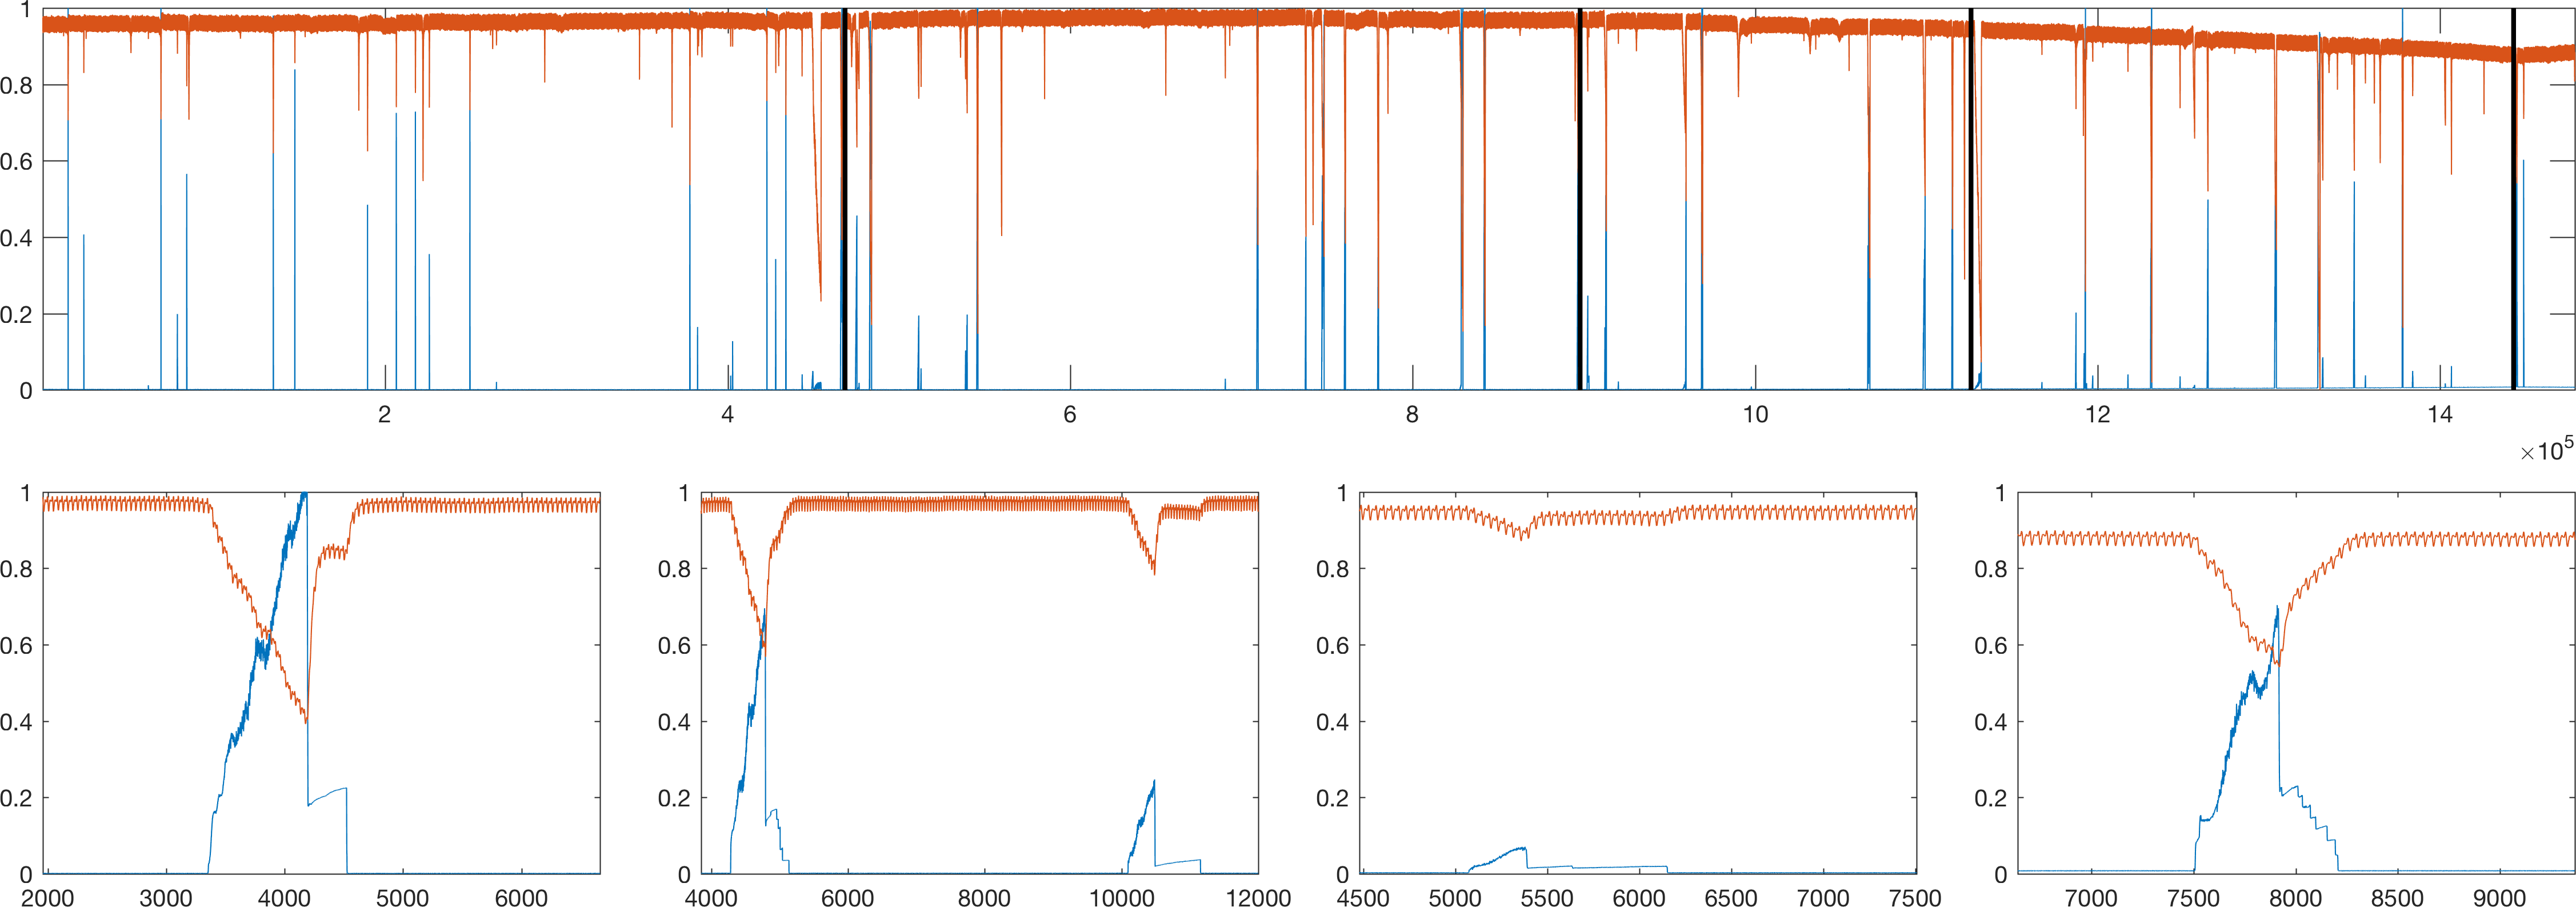
\includegraphics[width=1\linewidth]{Scan_SolitonSpot}}
\end{minipage}
\caption{Сканирование лазером большой мощности 1 ОСД резонатора из $MgF_2$. Сверху красным даны сигналы пропускания системы, синим - генерируемый свет (сигнал пропускания за вычетом отфильтрованного мощного сигнала накачки). Наблюдается большое количество оптических гребенок, генерируемых на разных семействах мод. Черным выделены несколько примеров мод с характерным для генерации солитонов ступеньками в сигнале генерируемого света (даны в увеличенном масштабе в нижнем ряду)}
\label{Scan_SolitonSpot}
\end{figure}

Был проведен эксперимент по одновременной генерации солитонов на разных семействах мод (Рис. \ref{Figure1_V1_c}), т.ч. одно семейство мод накачивалось лазером, а другое семейство боковой линией амплитудной модуляции этого лазера. Использовался амплитудный модулятор с 1 боковой линией, сигналы от которых усиливались в эрбиевом волоконном усилителе. Связь с резонатором осуществлялась через одно растянутое волокно. Сигнал на выходе системы проходил через волоконный Брэгговский фильтр для подавления мощного сигнала накачки и анализировался на оптическом спектроанализаторе и быстром фотодиоде с помощью анализатора сигналов. Частота сигнала, подаваемого на модулятор выбиралась так, чтобы на картине сигнала генерируемого света, ступеньки от двух нелинейных резонансов совпадали, их пересечение является областью одновременного существования солитонов (Рис. \ref{Figure2}). Далее использовалась стандартная техника настройки на солитонный режим, когда подается однократный пилообразный сигнал, который быстро перестраивает лазер в область существования солитонов. Использовалась активная температурная стабилизация резонатора с помощью элемента Пельтье, установленного под подставку под резонатора, диодный датчик температуры, который был закреплен на подставке (не на резонаторе, что вносило дополнительную задержку при стабилизации) и PID регулятор. Температура резонатора стабилизировалось с точностью до 10 мК. Стабилизация отстройки частоты лазера проводилась методом PDH.

\begin{figure}[ht]
\begin{minipage}[ht]{1\linewidth}
\center{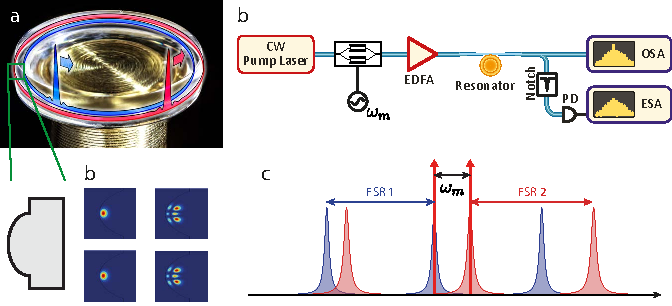
\includegraphics[width=0.75\linewidth]{Figure1_V1_c}}
\end{minipage}
\caption{(а) Фотография резонатора $MgF_2$ диаметр 5.5 мм, радиус кривизны боковой поверхности 80 мкм, схематично изображены 2 солитона на различных семействах мод, распространяющихся в одном направлении, ниже даны примеры распределения поля внутри МШГ для 2х разных семейств мод, (b) Схема экспериментальной установки: CW pump laser - волоконный перестраиваемый лазер непрерывной мощности, волоконный амплитудный модулятор с 1 боковой линией, EDFA - эрбиевый волоконный усилитель, резонатор из (а), Notch - волоконный Брэгговский фильтр, PD - быстрый фотодиод, OSA - оптический спектроанализатор, ESA - анализатор спектра электрических сигналов. (с) концептуальная схема эксперимента, красным и синим изображены разные пространственные семейства мод в одном резонаторе, имеющие разные ОСД FSR1 и FSR2, расстояние между накачиваемыми двумя модами $\omega_m$ выбирается как частота модуляции.}
\label{Figure1_V1_c}
\end{figure}

\begin{figure}[ht]
\begin{minipage}[ht]{1\linewidth}
\center{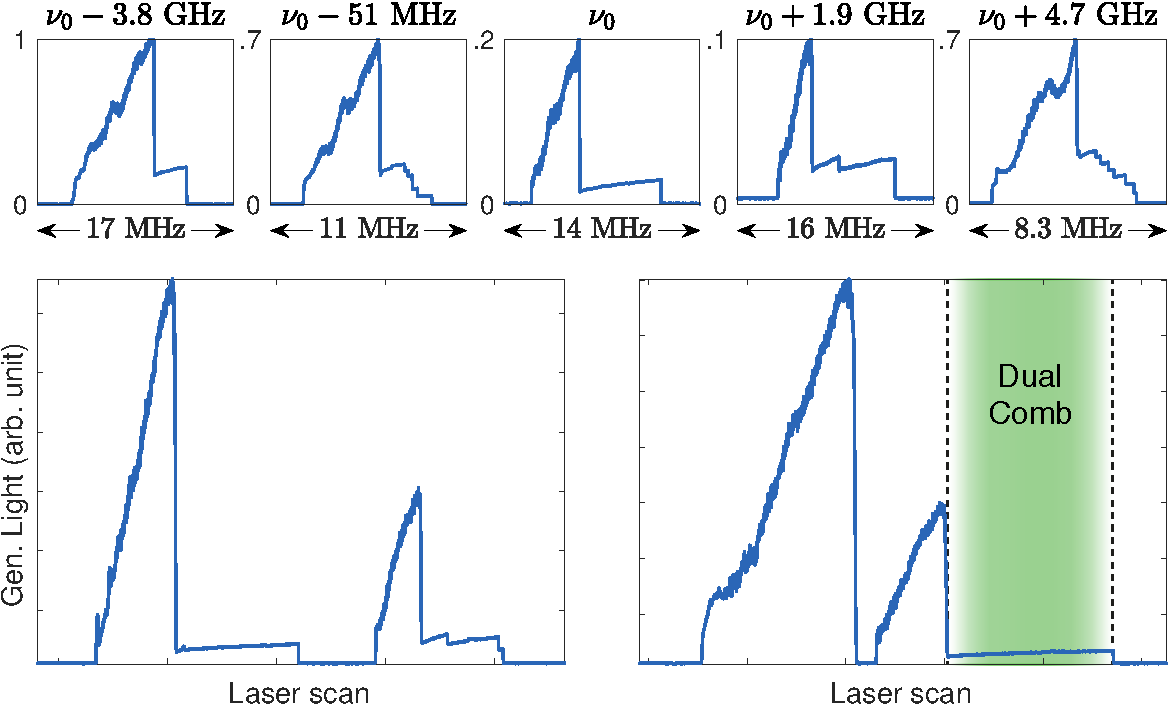
\includegraphics[width=0.5\linewidth]{Figure2}}
\end{minipage}
\caption{Сверху показаны сигналы генерируемого света для разных семейств мод, содержащие характерные солитонные ступеньки, даны отличия собственных частот для этих мод от выбранной центральной. Масштаб по вертикальной оси разный. Внизу показан метод совмещения солитонных ступенек при изменении частоты модуляции. Зеленой областью показан диапазон отстройки, при котором одновременно могут существовать солитоны на обоих семействах мод.}
\label{Figure2}
\end{figure}

В ходе эксперимента удалось одновременно настроиться на оба солитона на разных семействах мод и стабилизировать отстройку частоты лазера, т.ч. солитоны существовали несколько часов. На рис. \ref{Co_Scheme_results} приведены экспериментальные результаты по одновременной генерации односолитонных режимов на двух разных семействах мод в одном резонаторе. Амплитуда лазера и 1 линии боковой модуляции были сделаны одинаковыми, частота модуляции составила 4.2817 ГГц, на этой же частоте наблюдалась результирующая гребенка в СВЧ диапазоне. Расстояние между линиями СВЧ гребенки составила 655 кГц, что равно разнице между частотами повторения солитонов на двух семействах мод. С помощью быстрого фотодетектора и осциллографа был измерена интерферограмма, которая подтвердила, что в результате мультигетеродинирования двух оптических солитонов образовался импульс в СВЧ диапазоне, огибающая которого соответствует огибающим в оптическом диапазоне. Также была измерена ширина одной нецентральной линии СВЧ гребенки, она составила 100 Гц (лимитирована разрешением прибора), что говорит об очень высокой взаимной когерентности оптических солитонов, которая в данном случае определяется стабильностью подаваемого СВЧ сигнала на модулятор и качеством стабилизации частоты отстройки лазера.

Таким образом был продемонстрирован перенос 35 нм оптической гребенки с центром на 1554 нм в СВЧ область с центром на 4.28 ГГц и шириной около 200 МГц. Такой источник двойной гребенки может использоваться для спектроскопии и быстрого измерения расстояний.

\begin{figure}[ht]
\begin{minipage}[ht]{1\linewidth}
\center{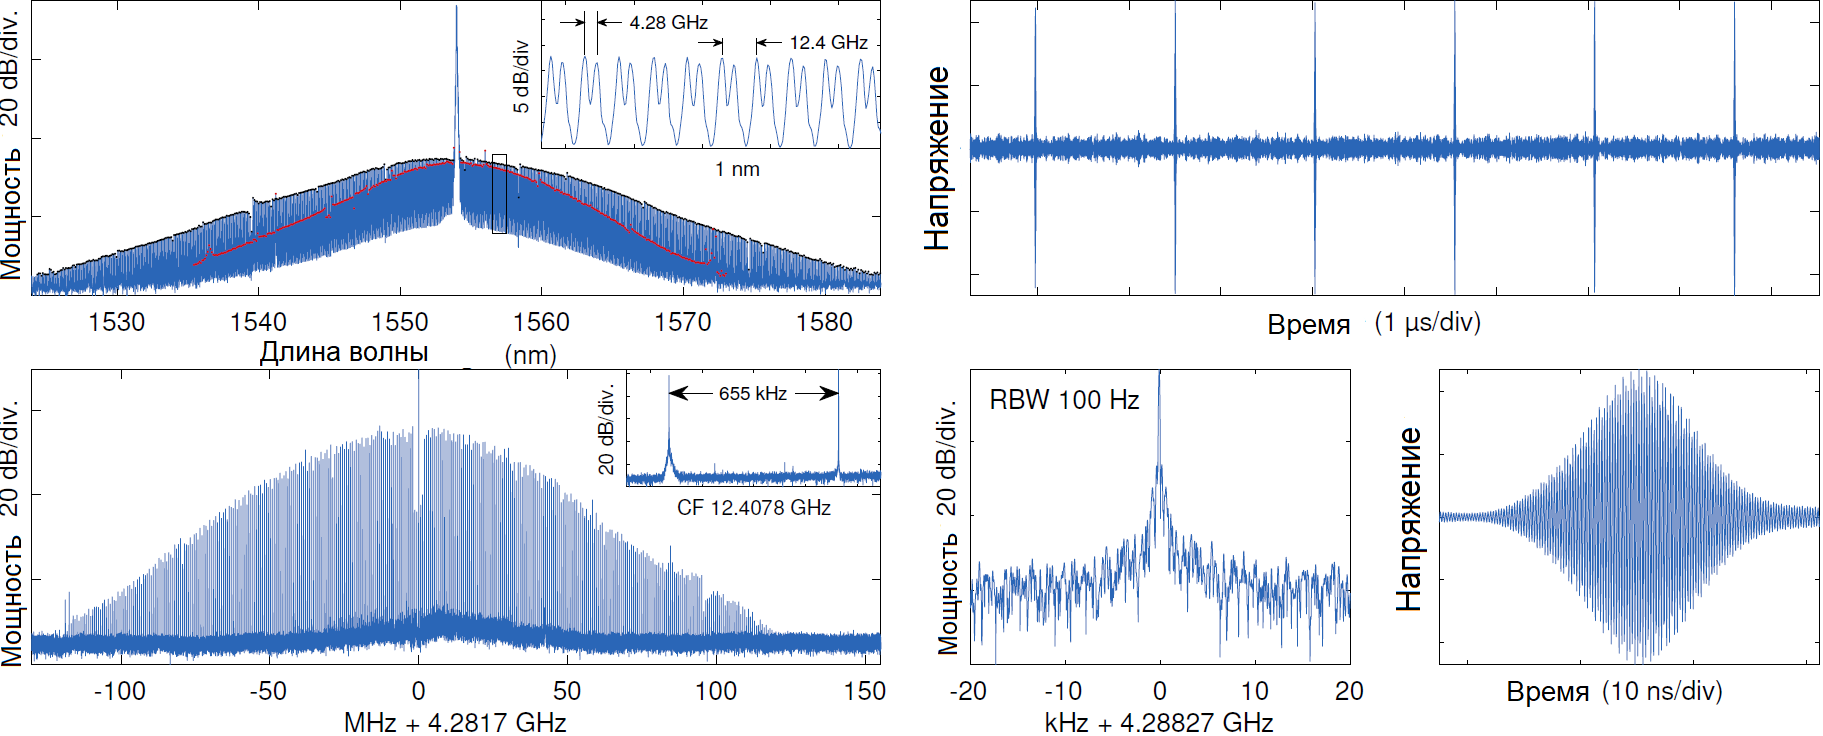
\includegraphics[width=1\linewidth]{Co_Scheme_results}}
\end{minipage}
\caption{Экспериментальные результаты одновременного возбуждения односолитонных режимов на двух разных семействах мод в 1 микрорезонаторе. (а) суммарный оптический спектр односолитонных режимов, красной линией помечена огибающая второго солитона, на вставке представлены отдельные линии двух солитонов. ОСД резонатора 12.4 ГГц, расстояние между несущими 4.28 ГГц. (b) результирующий сигнал биений двух солитонов - СВЧ гребенка с расстоянием между линиями 655 кГц, которое соответсвует разнице между ОСД семейств мод, на вставке изображены сигналы частот повторения двух солитонов, (с) сигнал последовательности результирующих СВЧ импульсов, снятый быстрым осциллографом, (d) одиночная нецентральная линия СВЧ гребенки шириной около 100 Гц, (е) сигнал одиночного СВЧ импульса, соответствующий СВЧ гребенки}
\label{Co_Scheme_results}
\end{figure}

На рис. \ref{coscheme_different_types} приведены результаты генерации солитонов на другой паре семейств мод. Частота модуляции, равная разнице собственных частот мод из двух семейств, составила $4.9119$~ГГц, расстояние между ОСД семейств мод 9.2633~МГц, оно же являлось расстоянием между линиями СВЧ гребенки. В данном случае на одном семействе мод был достигнут односолитонный режим, а на другом многосолитонный. Хорошо видно совпадение огибающих оптического спектра солитонов и результирующего спектра СВЧ сигнала. Отметим видимый в этом эксперименте недостаток, при большом отличии ОСД между семействами мод, результирующая СВЧ гребенка перекрывается с собой, т.к. линии от мультигетеродинирования расположены вокруг центральных частот $\omega_m$ и $FSR-\omega_m$. Этот же недостаток может проявляться и при достаточно малых $\omega_m$.

Измерение стабильности индивидуальной линии \ref{single_line_stability_cp} говорит о хорошей стабилизации частоты лазера накачки и температуры резонатора.

\begin{figure}[ht]
\begin{minipage}[ht]{1\linewidth}
\center{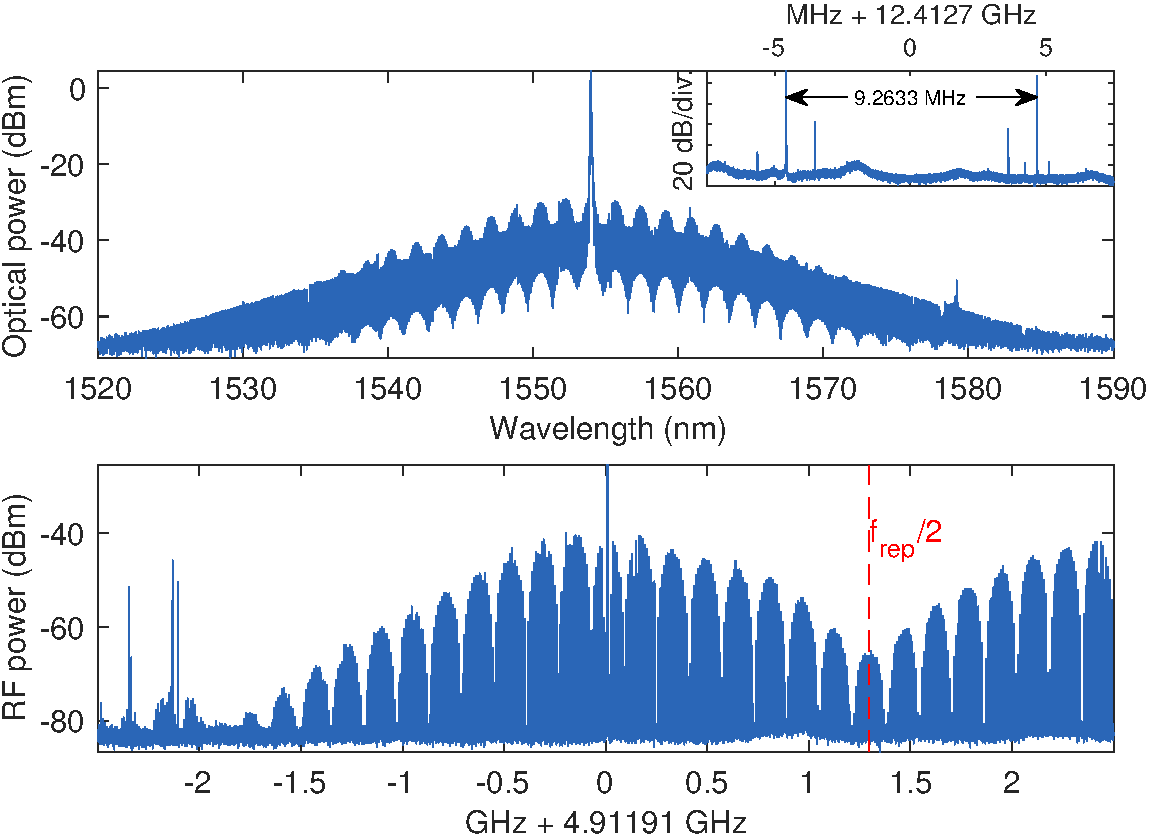
\includegraphics[width=0.75\linewidth]{coscheme_different_types}}
\end{minipage}
\caption{Результаты генерации солитонов в одном направлении на другой паре семейств мод. (а) суммарный оптический спектр односолитонного режима на одном семействе мод и многосолитонного режима на другом семействе мод, на вставке показана разница между частотами повторений 9.2633~МГц, (b) результирующая CВЧ гребенка с центральной частотой 4.9119 ГГц, видно что гребенка перекрывается с собой на половине частоты повторонения солитонов, отмечено красной линией.}
\label{coscheme_different_types}
\end{figure}

\begin{figure}[ht]
\begin{minipage}[ht]{1\linewidth}
\center{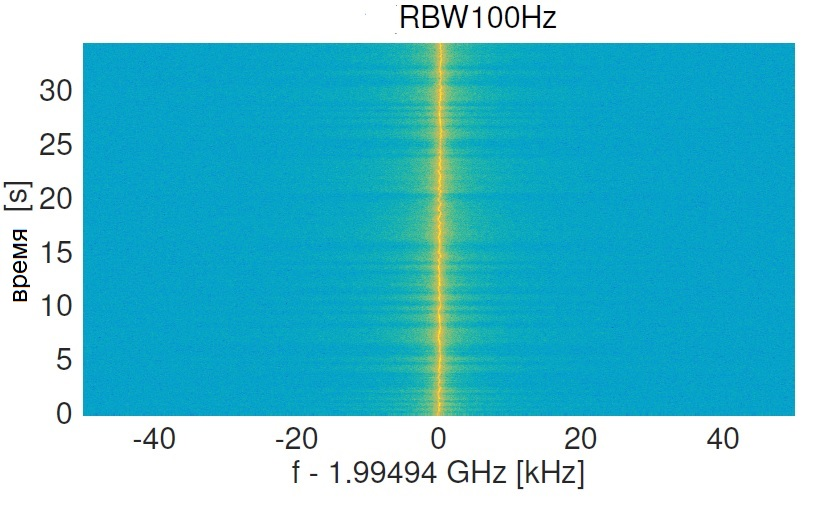
\includegraphics[width=0.5\linewidth]{single_line_stability_cp}}
\end{minipage}
\caption{Измерение стабильности индивидуальной линии СВЧ гребенки.}
\label{single_line_stability_cp}
\end{figure}

Отметим также технический недостаток схемы с двумя солитонами в одном направлении - сигнал ошибки схемы PDH несет информацию одновременно от обоих резонансов, что может мешать стабилизации, особенно при наличии эффекта пересечения мод хотя бы на одном солитонном резонансе.

Практическим для некоторых приложений недостатком схемы с двумя солитонами в 1 направлении является невозможность разделить эти солитоны (у них одна поляризация и близкие частоты линий), поэтому такая схема может не подойти, например, для фазово-чувствительной спектроскопии поглощения веществ. Отметим, что признаков взаимодействия солитонов в данном эксперименте обнаружено не было.

\subsection{Генерация солитонных оптических гребенок в одном резонаторе на разных семействах мод в противоположных направлениях}

Чтобы разделить солитоны из одного резонатора был проведен следующий эксперимент, в котором солитоны на разных семействах мод возбуждались в противоположных направлениях. Схема экспериментальной установки приведена на рис. \ref{Setup_CounterProp}. Волоконный перестраиваемый лазер непрерывной мощности усиливается эрбиевым усилителем, 0.1 мощности в одном плече после делителя модулируется амплитудным модулятором с одной боковой линией в таком режиме, что вся мощность перекачивается в эту боковую линию, далее сдвинутый по частоте лазерный сигнал усиливается и подается через оптический циркулятор в резонатор из $MgF_2$, другое плечо содержит 0.9 мощности исходного лазера и подается через другой циркулятор на тот же элемент связи - растянутое волокно. Третьи выходы двух оптических циркуляторов в такой конфигурации содержат свет, прошедший через резонатор в противоположных направлениях. Брэгговские волоконные фильтры используются для подавления мощных несущих. Далее полученные сигналы независимо подаются на оптические спектроанализаторы и могут быть сбиты на волоконном делителе и отправлены на быстрый фотодетектор для генерации СВЧ гребенки.

\begin{figure}[ht]
\begin{minipage}[ht]{1\linewidth}
\center{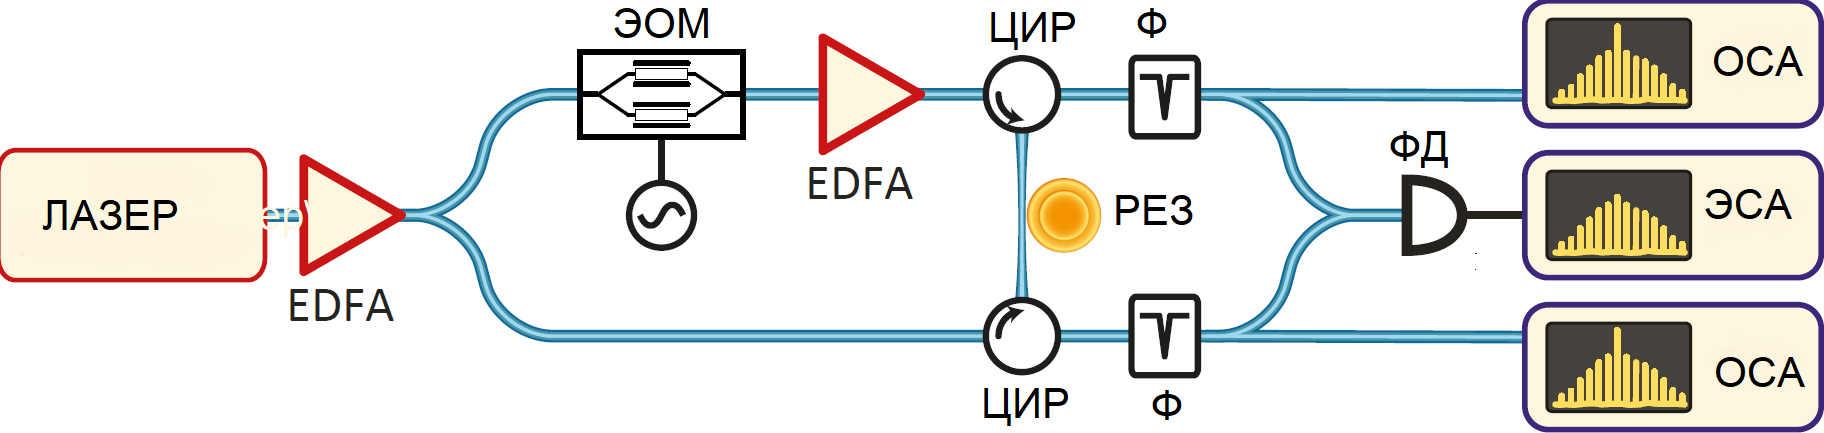
\includegraphics[width=0.75\linewidth]{Setup_CounterProp}}
\end{minipage}
\caption{Схема экспериментальной установки: CW pump laser - волоконный перестраиваемый лазер непрерывной мощности, волоконный амплитудный модулятор с 1 боковой линией, EDFA - эрбиевый волоконный усилитель, резонатор из (а), Notch - волоконный Брэгговский фильтр, PD - быстрый фотодиод, OSA - оптический спектроанализатор, ESA - анализатор спектра электрических сигналов, CIR - оптический циркулятор}
\label{Setup_CounterProp}
\end{figure}

В эксперименте мощность накачек в обоих плечах выравнивалась, а частота модуляции подбиралась так, чтобы совпадали солитонные ступеньки в сигнале генерируемого света, также как и в случае солитонов в 1 направлении на разных семействах мод. Использовался метод PDH стабилизации частоты лазера к моде резонатора. Также была задействована схема активной стабилизации температуры резонатора. Экспериментальные результаты приведены на \ref{counter_prop_results}. Красный оптический спектр имеет сильно выраженный пик на 1530 нм, вероятно, связанный с сильным эффектом пересечения мод. Результирующая картина СВЧ гребенки хорошо воспроизводит огибающие оптических спектров солитонов (однако присутствуют дополнительные компоненты на +70 МГц и -70 МГц, вероятно, связанные с техническими шумами). Результаты измерения девиации Аллана показывают, что разница частот повторений солитонов стабильнее, чем индивидульная частота биений для 1 солитона, что говорит о хорошей работе системы привязки PDH. Для того чтобы минимизировать флуктуации амплитуд индивидуальных линий СВЧ гребенки необходимо бороться с паразитными переотражениями в схеме после резонатора, иначе образуются дополнительные резонаторы типа Фабри-Перо, и избегать флуктуаций фазы света в плечах, уменьшая длину волокон и контролируя их температуру и механические вибрации.

Продемонстрированный метод генерации двойной гребенки в противоположных направлениях на разных семействах мод подходит для проведения фазочувствительной спектроскопии. Отметим, что признаков взаимодействия солитонов в данном эксперименте обнаружено не было.

\begin{figure}[ht]
\begin{minipage}[ht]{1\linewidth}
\center{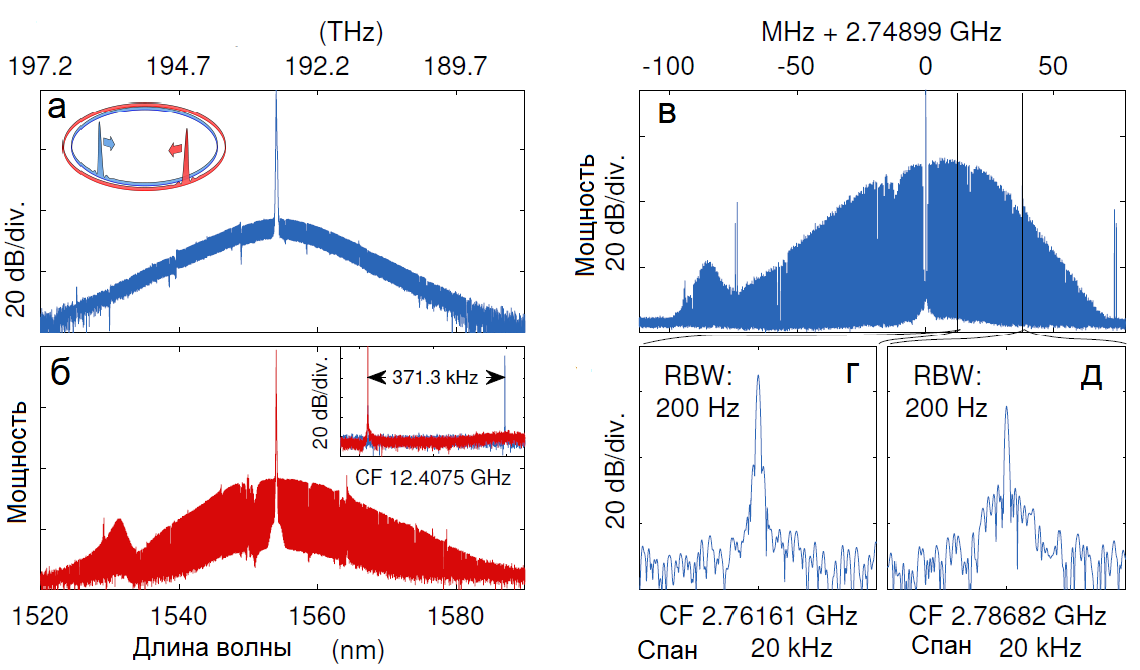
\includegraphics[width=1\linewidth]{counter_prop_results}}
\end{minipage}
\caption{Экспериментальные результаты возбуждения солитонов в противоположных направлениях в 1 резонаторе на разных семействах мод. (а,с) Оптические спектры односолитонных режимов, полученных на разных семействах. На вставке показаны наложенные друг на друга сигналы биений на частоте повторения солитонов. Разница в частотах повторений составила 371 кГц. (b) Результирующая СВЧ гребенка при совмещении потоков солитонов, распространяющихся в противоположном направлении, центральная частота совпадает с частотой модуляции 2.748 ГГц, расстояние между линиями 371 кГц, (d) измерение девиации Аллана частоты повторения для одного потока солитонов на 12.407 ГГц (красные точки) и для их разности (черные точки)}
\label{counter_prop_results}
\end{figure}

\subsection{Генерация солитонных оптических гребенок в одном резонаторе на одном семействе мод в противоположных направлениях}

Предложенный метод генерации солитонов в 1 резонаторе в противоположных направлениях применим не только при накачке разных семейств мод, но возможен и на одном семействе мод. Используя схему \ref{Setup_CounterProp} и экспериментальный метод из предыдущего раздела, возможно возбудить два солитона на 1 моде в противоположных направлениях \ref{cp_one_family}, для этого на амплитудный модулятор подается частота не выше максимальной отстройки, при которой существует солитон (типичные значения 5-20 МГц). Т.к. частота повторения солитонов зависит от отстройки частоты накачки от холодного резонанса, то при небольшом сдвиге накачки в прямом и обратном направлениях возможно образование результирующей СВЧ гребенки \ref{cp_one_family_dual_comb}. Важно отметить, что существует пороговое значение этой отстройки (частота на модуляторе менее 2 МГц), при которой частоты повторения солитонов строго совпадают и двойная гребенка не наблюдается. Также экспериментально обнаружено, что частоты повторений могут совпасть и при таком значении отстройки, когда возбуждаются сильные пересечения мод. Важно отметить, что использования одного лазера недостаточно, т.к. при 0 отстройке накачек друг относительно друга, частоты повторений совпадают.

Измеренная стабильность индивидуальных линий \ref{cp_one_family_stability} показывает сдвиг на 100 Гц за 60 сек, однако флуктуации амплитуды индивидуальных линий были высокими (Рис. \ref{cp_one_family_dual_comb} (b)), вероятной технически устранимой причиной являются сильные паразитные переотражения на коннекторах волокон волоконного делителя.

\begin{figure}[ht]
\begin{minipage}[ht]{1\linewidth}
\center{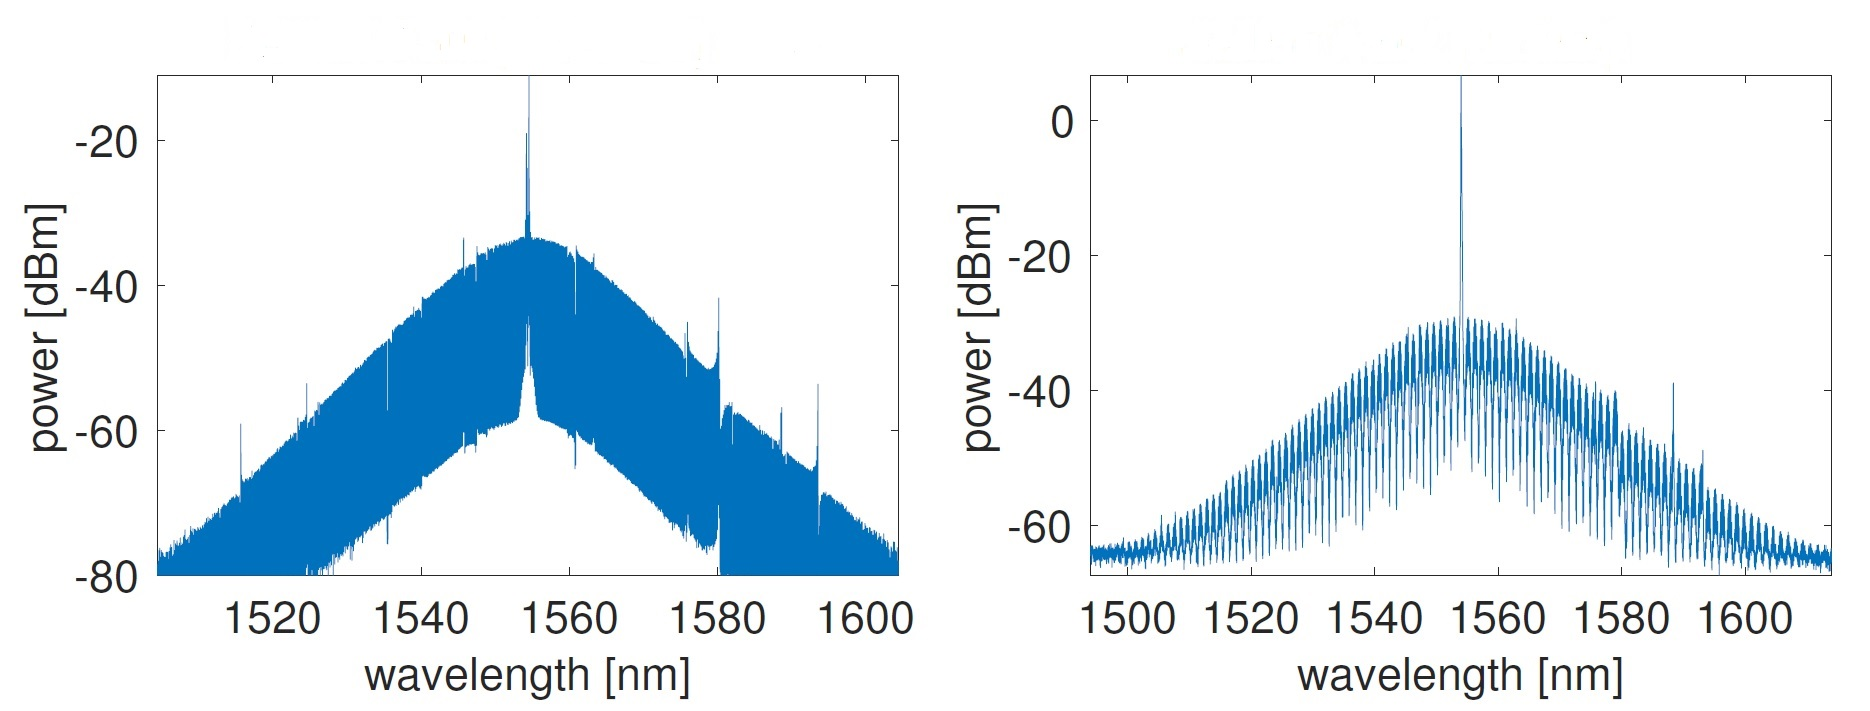
\includegraphics[width=0.7\linewidth]{cp_one_family}}
\end{minipage}
\caption{Экспериментальные результаты возбуждения солитонов в противоположных направлениях в 1 резонаторе на одном семействе мод. (а,b) Оптические спектры: односолитонный режим в одном направлении, многосолитонный режим в противоположном направлении на том же семействе мод.}
\label{cp_one_family}
\end{figure}

\begin{figure}[ht]
\begin{minipage}[ht]{1\linewidth}
\center{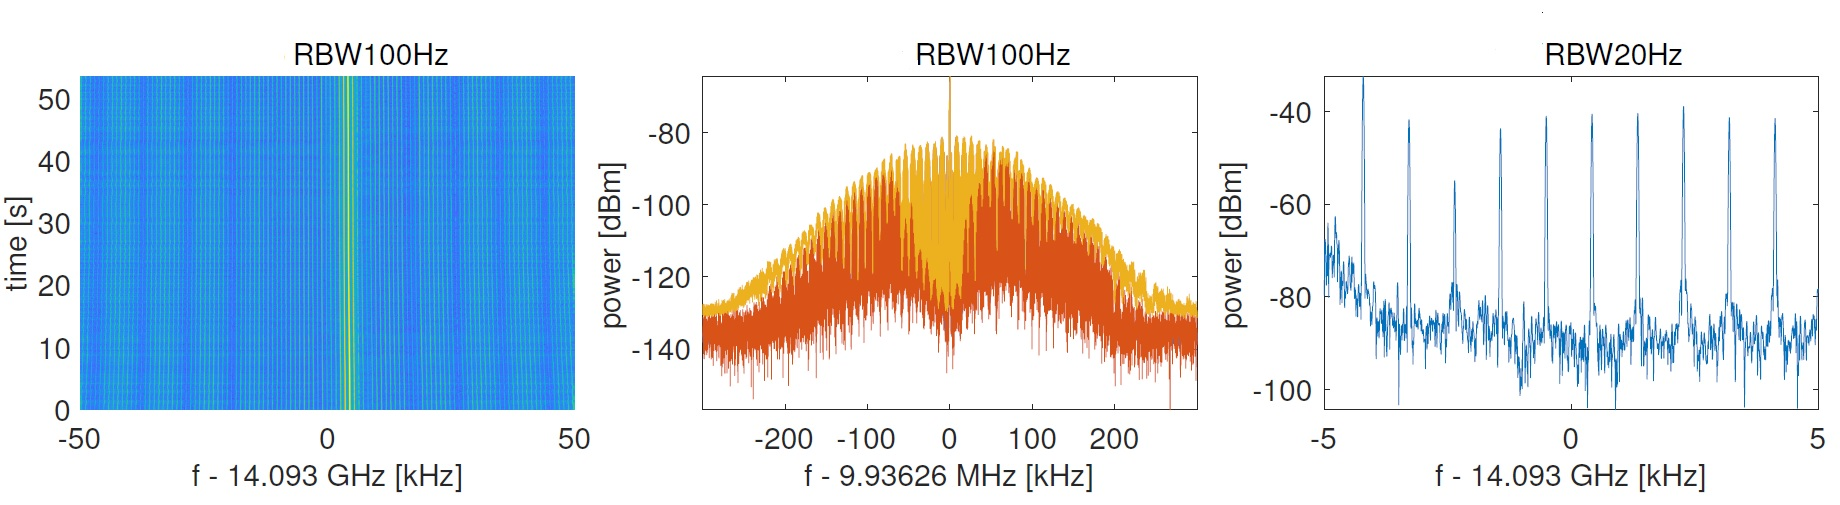
\includegraphics[width=1\linewidth]{cp_one_family_dual_comb}}
\end{minipage}
\caption{Результирующая СВЧ гребенка при совмещении потоков солитонов, распространяющихся в противоположном направлении, центральная частота совпадает с частотой модуляции 9.93 МГц, расстояние между линиями СВЧ гребенки порядка 1 кГц и растет с увеличением разности частот накачек. (а) стабильность результирующей гребенки, (b) спектр гребенки, желтым максимальное значение, красным - усредненное за 10 сек, (c) спектр индивидуальных линий результирующей гребенки}
\label{cp_one_family_dual_comb}
\end{figure}

\begin{figure}[ht]
\begin{minipage}[ht]{1\linewidth}
\center{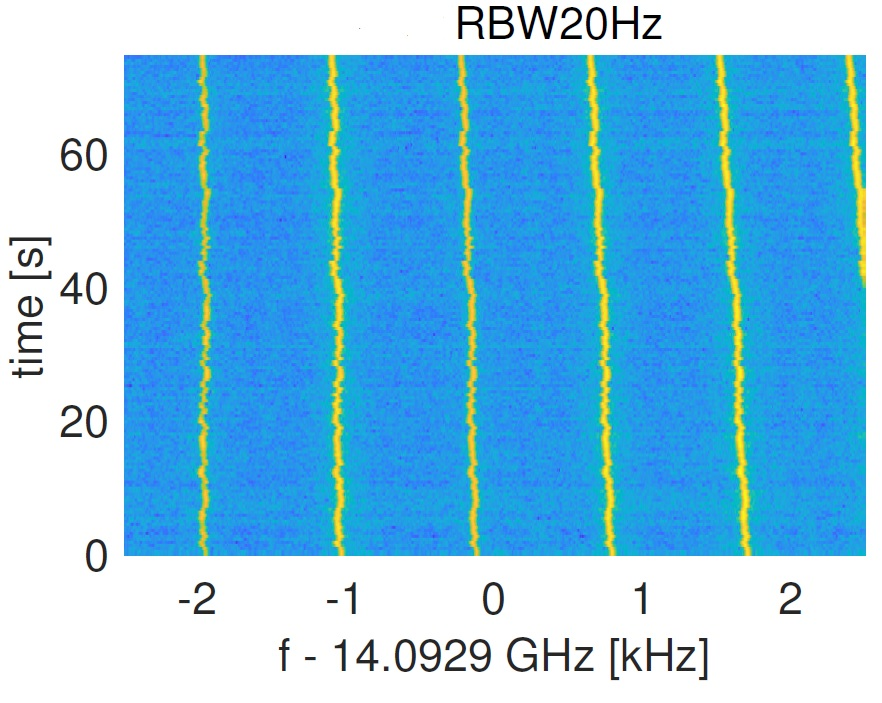
\includegraphics[width=0.5\linewidth]{cp_one_family_stability}}
\end{minipage}
\caption{Стабильность индивидуальных линий гребенки, полученной как биение двух солитонов, возбужденных на одном семействе мод в противоположных направлениях}
\label{cp_one_family_stability}
\end{figure}

Предложенный метод может быть удобен тем, что подходит для одномодовых резонаторов или резонаторов, не поддерживающих солитоны на разных семействах мод, а также тем, что не требует высоких частот, подаваемых на модулятор и быстрых фотодетекторов для регистрации двойных гребенок в СВЧ области.

%Сошлемся на все конференции \cite{confbib1,confbib2,confbib3,confbib4,confbib5,confbib6,confbib7,confbib8,confbib9,confbib10,confbib11,confbib12,confbib13,confbib14}
%\section{Экспериментальное наблюдение вынужденного рассеяния Рамана и Бриллюэна в кристаллических микрорезонаторах} 